\documentclass[a4paper]{article}

\usepackage[english]{babel}
\usepackage[utf8]{inputenc}
\usepackage{amsmath}
\usepackage{graphicx}
\usepackage[colorinlistoftodos]{todonotes}
\usepackage{caption}
\usepackage{pgfplots}
\pgfplotsset{width=10cm,compat=1.9}
\renewcommand{\thetable}{\arabic{section}.\arabic{table}}
\newcommand\T{\rule{0pt}{2.6ex}}       % Top strut
\newcommand\B{\rule[-1.2ex]{0pt}{0pt}} % Bottom strut

\title{PHY 4210-01 Senior Lab \\Lab M-1: Magnetic Field Mapping}

\author{Sarah Arends \\ 
        Jacquelyne Miksanek \\
        Ryan Wojtyla \\ \\
        Instructor: Jerry Collins II}

\date{February 7, 2019}

\begin{document}
\maketitle 

\begin{abstract}
%physics of experiment
%apparatus used
%what was measured
%Results
In this experiment the magnetic field inside a Helmholtz coil was measured and compared to theoretical calculations determined from the Smythe derivation of the Biot-Sarvat Law for a plane displaced from the central axis, with coordinates z, $\rho$, and $\phi$.When determining the magnetic field inisde a Helmholtz coil, a Hall probe is used to obtain the magnitude of the magnetic field at varrying positions inside the coil. Theoretically the magnetic field that is produced axially inside of the Helmholtz coil is of uniform magnitude.    
% second sentence of results still needed!!!
\end{abstract}

\newpage

\tableofcontents

\newpage

\section{Objective of the Experiment}
%A brief statement on the main purpose of the experiment
During this lab, the number of turns of wire inside a Helmholtz coil was determined for use in theoretical calculations. Then a 3-dimensional and 2-dimensional mapping of the magnetic field inside the Helmholtz coil was created in order to investigate the presence of a uniform field, running along its axial direction.

\section{Theory of the Experiment}
%A short presentation of the concepts and formulas related to the experiment.

% How a helmholtz coil produces a uniform field
Recall for a straight current-carrying wire, circular magnetic field lines are generated around the wire in accordance with the curling right-hand rule. The Helmholtz coil contains two regions of circularly wound wires. Due to the the circular symmetry, all components of each infinitesimal segment of the wire will cancel \textit{except} for that in the axial direction. In summary, a circular current produces a linear magnetic field.
% off-axis field point
The field point of the system has before been typically placed along the axis of the direction of the magnetic field, we will call this the z-direction. This was due to the ease of solving the Biot-Savart Law under these simple conditions, as the direction and strength of the magnetic field will follow along the z-axis of the system, which is where the field point is placed. When this is applied to the co-axial coils of the Helmholtz apparatus the evaluation of the Biot-Savart Law becomes too trivial. One then chooses the field point to be placed off of the z-axis as more information about the magnetic field of the coils can be determined. This is the more general scenario and thus more complex. The off axis form can be used for any point that is off of the z-axis, while the on axis is a specific and simplified form of the general case. The general form is best represented by Smythe's derivation of the Biot-Savart Law. 
\begin{align*} 
B_z = \frac{\mu_0IN}{2\pi}
\Big[&
    \frac{1}{\sqrt{(a+\rho)^2 + (a-z)^2}}
    \big[
        K_1 + \left(\frac{a^2 -\rho^2 - (a - z)^2}{(a-\rho)^2 + (a - z)^2} \right) E_1 
    \big]\\
    & + \frac{1}{\sqrt{(a + \rho)^2 + z^2}}
    \big[
        K_2 + \big(\frac{a^2 - \rho^2 - z^2}{(a - \rho)^2 + z^2}\big) E_2 
    \big] 
\Big]
\end{align*}
\section{Equipment Utilized}
%List principal pieces of apparatus used by manufacturer, model and serial number. When it may be important, list principal specifications of certain pieces of equipment (e.g. the focal length of an optical system, etc.)

%How hall effect probe works
A DC Gaussmeter (AlphaLab Model GM-1-HS) was connected to a Hall Effect Probe in order to measure the field strength inside the Helmholtz coil. The Hall Effect Probe contains a semiconductor junction that, when exposed to a magnetic field, produces a voltage proportional to the field strength.

%Position Controls
The position of the Hall Effect Probe can be modified in the $\rho$ direction by sliding the ruler bar through the acrylic cube shown in figure \ref{diagram}. The position can be modified in the $\phi$ direction by rotation the ruler bar about the central pole. However, for the sake of this experiment, this did not have to be modified because measurements were taken in a single $\rho , z$ plane. The $z$ coordinate was modified by sliding the acrylic cube and ruler bar up and down the central pole.

%Labeled sketch of the experimental setup
\begin{figure}[h]
\centering
% uncomment the line below to add image
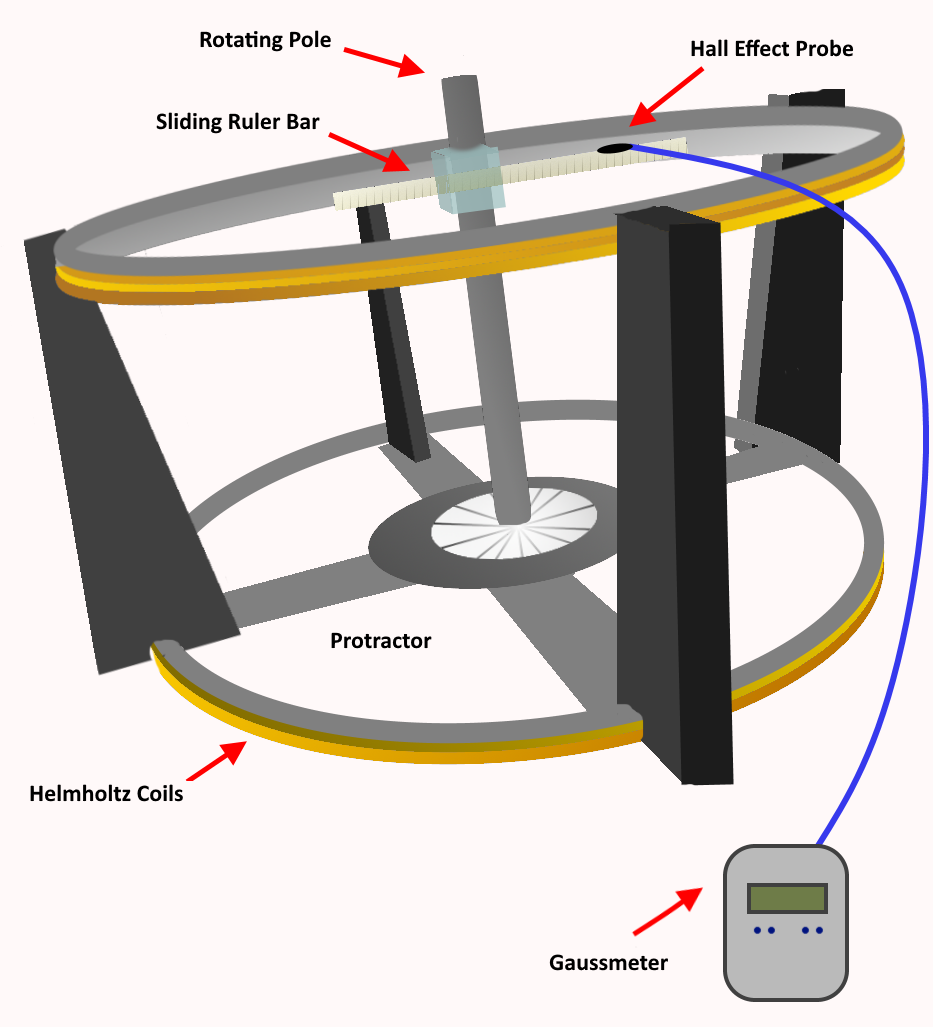
\includegraphics[width=0.5\textwidth]{helmholtz_diagram.png}
\captionof{figure}{Two concentric Helmholtz coils seperated by a distance equal to their radius. Rotating pole and sliding ruler allow for modification of the probe's position.}
\label{helmholtz_diagram}
\end{figure}


\section{Procedure}
% Describe in writing and provide a detailed sketch of the equipment used to measure the axial field in the coil.




%Describe the main steps in the experimental procedures. Be sure to include any precautions. Sufficient details should be given such that another student can follow and do the experiment.
Note that, per suggestion of the laboratory manual, the procedural steps of this experiment have been omitted. The discussion section provides sufficient detail on what actions were taken.

\subsection{Data Analysis}
%Graphs, figures, and tables with captions
%Results with error analysis
%Calculate discrepancies from theory

% Calculating

%Theoretical calculations of axial field strength

% 3D plot (theoretical)

% 2D plot (theoretical)

% 3D plot (exp)

% 2D plot (exp)

% Calculating discrepancies

% 3D plot discrepancies 

% 2D plot discrepancies

\section{Results}
%Discuss results and uncertainties
%Compare results with theory
%Approximations to theory


% Determine span of uniform region with 1percent margin and 5percent margin

% Compare B field in different direction, can we say field is axial
\subsection{Comparing the directions of the Magnetic Field}
When measuring at a probe height of a/2 (16cm), where 'a' is the separation distance between the coils, 
the strength of the magnetic field in the 'z' direction was measured to be -3.13 Gauss. When measuring t
he magnetic field in the 'z' direction at a probe height of 5cm, the magnetic field strength was measure
d to be -3.28 Gauss. These results follow with the theory as it is expected that the magnetic field is p
ropagated in the 'z' direction. The measured magnetic field strength for the $\rho$ direction was -0.46 
and -0.05 Gauss for a probe height of 16cm and 5cm respectfully. The measured magnetic field strength fo
r the $\phi$ direction was -0.51 and -0.31 Gauss for a probe height of 16cm and 5cm respectfully. For a 
probe height of 16cm the percentage for the magnitude of the magnetic field that is measured to be in th
e $\rho$ direction is 14$\%$ while the percentage for the magnitude of the magnetic field that is measur
ed to be in the $\phi$ direction is 16$\%$. For a probe height of 5cm the percentage for the magnitude o
f the magnetic field that is measured to be in the $\rho$ direction is 1$\%$ while the percentage for th
e magnitude of the magnetic field that is measured to be in the $\phi$ direction is 9$\%$.The magnetic f
ield produced by the Helmholtz coils should be directed along the 'z' axis. These small measuredvalues f
ollow the aforementioned theoryand we can determine that the magnetic field produced by the Helmholtz c
oil is indeed axial. Furthermore, we can determine thatthe magnetic field is axial along the 'z' direct
ion.
\section{Conclusion}
%Brief summary, discussion of results and theory

\end{document}
